%!TEX root = ../Studienarbeit.tex

%!TEX root = ../Studienarbeit.tex


\section{Hardwarerealisierung}

Für einen optimalen Vertreibungseffekt werden verschiedene Aktoren im System verbaut. Die einzelnen Geräte werden alle über eine externe Energieversorgung, beziehungsweise Batterie betrieben. Bei der Wahl der Batterie, ist ein wichtiges Kriterium, wie lange das System ohne Energiezufuhr funktionsfähig bleibt.
\\
Dabei wurde berücksichtigt, wie viel das System im Normalverbrauch ohne Einschalten der Aktoren verbraucht. Eine grobe Schätzung ergab, dass das System ungefähr 10 $\pm$ 2 Watt pro Stunde verbrauchen würde. Aus diesem Grund fiel die Wahl auf eine 50 Ah Autobatterie von \textit{BlackMax} \cite{Autobatterie} gefallen. Diese Batterie bietet ausreichend Kapazität, um das System über zwei Tage mit Energie zu versorgen.
\\
Ein weiterer Entscheidungsgrund für die Autobatterie ist der Strombedarf der Geräte. Wie nachfolgend beschrieben, kann die Wasserpumpe im laufenden Zustand bis zu 16 Ampere Strom beziehen. Viele leichte und kleine Batterien könnten langfristig durch diese Belastung Schaden nehmen. Da Autobatterien eine hohe Belastungsgrenze haben und hohe Ströme ermöglichen, sind sie daher für den Prototypen besser geeignet.

Für die Unterbringung aller Teile wird eine 40x55x30 \ac{CM} große Aluminiumkiste verwendet. Die Aluminiumkiste ist witterungsbeständig, und die Wärmeentwicklung im Inneren kann weitestgehend vernachlässigt werden. Aluminium hat nämlich eine gute Temperaturleitfähigkeit und kann somit einen Wärmestau verhindern. Dabei ist auch der Empfehlung aus einem \textit{Autodesk Instructables}-Projekt folge geleistet worden. In diesem Projekt wurde eine bewegungsausgelöste "`Wasserpistole"' aufgebaut. Allerdings war bei dem \textit{Instructables}-Projekt eine Vertreibung von Rehen vorgesehen, die sonst die Rosen im Garten aufgegessen hätten. Das Ziel dieser Arbeit ist es aber Waschbären und andere Kleintiere zu vertreiben, daher sind hier noch weitere Aktoren eingebaut. Zudem ist das \textit{Instructables}-Projekt nicht autark und portable, da es mit Strom und Wasser mittels Hausanschluss versorgt worden ist. \cite{watergun_dude}

Die eingebauten Bauteile werden nachfolgend beschrieben.

\subsection{Blitzlicht}

Für den Einsatz eines Abschrecklichtes mit Blitzlichtfunktion werden zwei LED-Scheinwerfer der Marke \textit{NAIZY} verwendet. Die Scheinwerfer sind für den Einsatz als Erweiterungsleuchten für Geländefahrzeuge gedacht. Sie sind wasserdicht und für den Außeneinsatz geeignet. Mit 1600 Lumen und grellweißem Farbton erzielen sie einen hohen stroboskopischen Effekt, mit dem die Tiere abgeschreckt werden. Aufgrund dieser Charakteristiken und des geringen Energieverbrauchs von 18 Watt sind sie für das Abschrecksystem sehr gut geeignet. \cite{am_licht}

Die beiden LED-Scheinwerfer sind an den beiden oberen Ecken der Box befestigt. Sie werden mit Transistoren durch den Mikrocontroller gesteuert. Um einen Gewöhnungseffekt zu vermeiden, sind die Scheinwerfer mit 0,5 bis 10 Hz beschaltet. Die Frequenz und Schaltung der Scheinwerfer wird dynamisch angepasst. Im Schaltbild aus Abbildung \ref{diag:lights_diagram} wird die Verwendung eines MOSFET-Treiberbausteins erkennbar. Der Treiber ermöglicht das Beschalten der Scheinwerfer mit höherer Leistung, als es mit dem Arduino möglich wäre. Der Treiber verfügt über eine zusätzliche Masse-Leitung, die mit dem Arduino verbunden ist. Dadurch ist es möglich den Strom zu schalten, auch wenn der Signalgeber und \textit{DC-Out} nicht die selbe Masse haben. \cite{mosfets_am}

\begin{figure}[h]
    \centering
    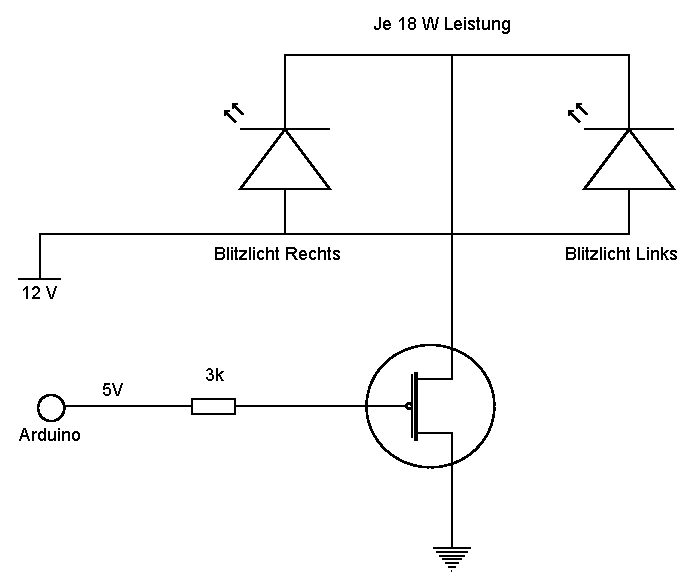
\includegraphics[width=0.6\textwidth]{images/lights_diagramm.pdf}
    \label{diag:lights_diagram}
    \caption{Schaltbild der Abschreckleuchten mit Ansteuerung}
\end{figure}

\subsection{Wasserversorgung und Pumpeneinheit}

Für den Einsatz eines \textit{Abschusssystems} mit Wasser benötigt das Abschrecksystem weitere Komponenten, welche folgend beschrieben werden.

\subsubsection{Pumpe} \label{cap:pumpe}

\comment{Bild mit Spritzschutz von Seite aus}

Auch wenn die Aluminiumkiste witterungsbeständig ist, schützt sie nur mäßig vor kalten Temperaturen. Dabei können viele Wasserpumpen schaden nehmen, wenn sie über den Winter draußen sind. Bei Membranpumpen ist dies ein kleineres Problem. Die zu den Oszillationsverdrängerpumpen gehörende Pumpenart ist außerdem sehr wartungsfreundlich und außerordentlich robust. Sie können daher selbst schwierigen Bedingungen und Temperaturumschwünge leicht standhalten.
\\
Ihre Funktionsweise beruht darauf, den \textit{Schöpfraum} periodisch zu vergrößern und zu verkleinern. Dadurch erzielen sie ihre Pumpwirkung und werden durch ihre Robustheit, Ölfreiheit (keine Verschmutzung der zu fördernde Flüssigkeit oder Gase) und Wartungsfreundlichkeit auch in chemischen Laboranwendungen verwendet. \cite{Jousten2018}

Für die Auswahl einer geeigneten Pumpe kamen zudem die Anforderungen an Fördermenge und Druck. Sprinkleranlagen werden wie in Kapitel \ref{sprinkler} beschrieben mit einem Gartenschlauch betrieben und können mit dieser Versorgung eine Reichweite von 10 Metern erreichen. Durch einen Hausanschluss fließen üblicherweise 20 Liter Wasser pro Minute mit einem Druck von etwa 4 Bar.\\
Die eingesetzte Pumpe von \textit{SEAFLO} hat eine maximale Fördermenge von 17 Liter pro Minute und kommt dadurch nahe an diesen Richtwert ran. Dabei nimmt sie bis zu 16 Ampere Strom auf. Auch bei dieser Leistungsaufnahme von über 190 Watt können die MOSFET-Treiber, die zum An- und Ausschalten der LED-Scheinwerfer verwendet werden, genutzt werden. Sie sind angegeben mit einer Dauerbelastung von 15 Ampere und mit Kühlung bis zu 30 Ampere. Da die Treiber nur für kurze Dauer eingeschaltet werden, ist eine zusätzliche Kühlung nicht nötig. \cite{mosfets_am,seaflo_pump}

Der Aufbau ist ähnlich zu dem Schaltbild \ref{diag:lights_diagram}. Allerdings wird zusätzlich eine Schutzdiode benötigt. Da Pumpen durch den internen Betrieb mittels Elektromotor eine induktive Last bilden, kann bei hartem Ein- und Ausschalten der MOSFET-Treiber durch Spannungsstöße Schaden nehmen \cite{induktive_last_diode}. Daher wird eine Schottky-Diode parallel zur Last eingebaut. Dies verhindert ein Aufbauen zu hoher Spannung, durch der der Transistor Schaden nehmen könnte. Schottky-Dioden eignen sich besonders gut für den Einsatz, da sie nur wenig Leistung aufnehmen und dadurch energiesparend sind. \cite{induktive_last_diode,am_schottky}

\subsubsection{Versorgung mit Wasser}

Damit die Pumpe mit Wasser versorgt werden kann, muss ein Wassertank in das System integriert sein. Allerdings ergeben sich dadurch verschiedene Probleme.
\\
Das größte Problem, das gelöst werden muss, ist die Unterbringung des Wassertanks. Durch den Einbau der verschiedenen Aktoren sowie der Autobatterie wurde in der Aluminiumkiste bereits viel Platz verwendet. Ein speziell an den verfügbaren Platz angepasster Tank kann zudem nicht mittels 3D-Drucker hergestellt werden, da die Drucke nicht wasserdicht sind. Ein herkömmlicher und einbaubarer Wassertank könnte daher nur wenige Liter fassen.

Ein weiteres Problem betrifft die Dichtigkeit des Tanks und der Pumpe. Beim Transport der Aluminiumkiste könnte eine große Menge Wasser leicht austreten. Aufgrund der Leitfähigkeit des Wassers könnten die Elektronikkomponenten Schaden nehmen. Dies wäre jedoch nicht so gravierend, da die Elektronik lediglich durchbrennen und der Stromkreislauf unterbrochen würde. Allerdings besteht bei der Aluminiumkiste die Gefahr, dass sie vollständig unter Strom gestellt wird. Dadurch würde sogar eine potenzielle Lebensgefahr entstehen, wenn man die Kiste berührt.
\\
Um die Sicherheit zu erhöhen, wird der Wassertank deshalb außerhalb der Kiste platziert und der Zulauf erfolgt durch eine seitliche Öffnung an der Kiste. Die Pumpe befindet sich jedoch weiterhin innerhalb der Kiste, um sie vor den äußeren Witterungsbedingungen zu schützen. Sie wird durch einen gedruckten Spritzschutz räumlich von den anderen Aktoren und der Spannungsversorgung getrennt. Der 3D-Druck ermöglicht jedoch keinen vollständigen Schutz, da er nur gegen geringe Wassermengen dicht hält. Spritzwasser und kleinere Leckagen durch die Pumpe können jedoch bewältigt werden.
\\
Vor dem Einbau in die Kiste wurde ein Dichtigkeitstest der Pumpe und des Spritzschutzes durchgeführt. Dabei traten nur bei bestimmten Bedingungen, wie dem seitlichen Legen oder Schütteln der Pumpe, geringe Mengen Wasser aus der Pumpe aus. Daher sollte der gedruckte Spritzschutz einen ausreichenden Schutz bieten.

\subsection{Mikrocontroller}

Durch die derzeitigen Liefermangel an Mikrocontrollern ergab sich die Auswahl eines passenden Mikrocontrollers für den Einsatz im Abschrecksystem ebenfalls als schwierig.\\
Getestet worden sind drei verschiedene Controller mit unterschiedlichen Erfolg, welche hier beschrieben werden.

Eine weitere Anforderung an das Abschrecksystem besteht darin, den Einsatz von \textit{Stereo Vision} für das korrekte Zielen zu ermöglichen. Alle drei Mikrocontroller sind daher mit zwei \ac{CSI}-Anschlüssen ausgestattet. Dies war von besonderer Bedeutung, da Multi-Camera Adapter wie von \textit{ArduCam} (\cite{arducam_multicam}) und auch USB-Kameras keine ausreichende Zeitsynchronität und Anpassbarkeit an das System ermöglichen. Nicht synchronisierte Kameras verfälschen die Tiefenberechnung sehr. Ein genaues Zielen wäre demnach nicht länger möglich wie aus der Arbeit von Shimizu und Co.hervorgeht. \cite{time_delay_sv}.
\\
Durch den direkten Anschluss an die \ac{CSI}-Anschlüsse wird dieses Delay minimiert. Die Mikrocontroller unterstützen teilweise die zeitgleiche Aufnahme von Bildern auf beiden \ac{CSI}-Anschlüssen. Im Falle des \textit{Jetson Nano}s ist eine Zeitsynchronität jedoch nicht vollständig gewährleistet. Dies geht aus dem \textit{ArduCam} Artikel von \cite{arduCam_sync_b01} hervor. Ein eigener Test ergab jedoch, dass die Kameras ausreichend synchron Bilder aufnehmen. Die Tiefenberechnung wäre demnach nicht zu stark beeinträchtigt, wie es mit dem \textit{MultiCam} Adapter der Fall wäre.

Um die Versorgungsspannung der 12V Autobatterie nutzen zu können, wird ein Spannungswandler benötigt, da die Mikrocontroller mit 5V betrieben werden. Der Spannungswandler muss in der Lage sein, kurzfristig eine ausreichende Leistung bereitzustellen. Bei der Objekterkennung können für einen kurzen Zeitraum hohe Leistungsabfragen entstehen. Wenn die Leistung dann nicht schnell genug bereitgestellt werden kann, kann es zum Zwangsabschaltungen des Mikrocontrollers kommen. Dadurch könnte auch der Controller selbst Schaden nehmen.
\\
Beim Aufsetzen und Testen des Jetson Nanos kam es wiederholt zu Stromabschaltungen. Der Nano wurde dabei mit einem Raspberry Pi Netzteil betrieben, das eine angegebene Leistung von 12,5 Watt hatte und daher für den Einsatz geeignet schien. Jedoch traten bei hohen Anforderungen, wie der gleichzeitigen Objekterkennung auf beiden Kameras, dennoch Stromabschaltungen auf. Im Gegensatz dazu traten beim Betrieb mit dem Spannungswandler und der Autobatterie keine unerwünschten Abschaltungen auf. Dies lag vermutlich daran, dass der einstellbare Spannungswandler von \textit{AzDelivery} laut den Angaben in \cite{am_spannungswandler} bis zu 60 Watt Leistung für den Mikrocontroller bereitstellen kann.

\subsubsection{Radxa \ac{CM} 3}

Durch den Liefermangel bestimmt waren Ende 2022 keine der nachfolgend beschrieben Mikrocontroller verfügbar. Daher ist das vom chinesischen Startup Radxa vertriebene \textit{Radxa Compute Module 3} für den Einsatz im Abschrecksystem getestet worden. Der Mikrocontroller zeichnet sich besonders durch die eingebaute \ac{NPU} sowie die verwendete Hardware wie \ac{SATA}-/USB 3.0-Anschlüsse und die Anzahl von 50 \ac{GPIO}-Pins aus. \cite{radxa}

Allerdings war das eigens für das \ac{CM} 3 konzipierte \textit{IO Board} zum Zeitpunkt der Untersuchung nicht erhältlich. Laut \textit{Radxa} ist das \ac{CM} 3 jedoch kompatibel mit dem \textit{\acl*{RPi} 4 IO Board}. Mit diesem Board kann das \ac{CM} 3 jedoch nur mit eingeschränkter Hardware genutzt werden.
\\
\textit{Radxa} bietet ein eigenes Betriebssystem für die Verwendung mit dem \ac{RPi} IO Board an. Bei der Einrichtung des Systems traten jedoch bereits Probleme auf. Zunächst konnte der \ac{eMMC}-Speicher nicht erfolgreich geflasht werden. Nur mit erhöhtem Aufwand war die Inbetriebnahme möglich.
\\
Im weiteren Betrieb traten weitere Probleme auf. Verschiedene Anwendungen und die Steuerung der Hardware (wie Kameras und \ac{GPIO}-Pins) waren sehr fehleranfällig und stürzten wiederholt ab.
\\
Auch konnte die \ac{NPU} des \ac{CM} 3 leider nicht mit den gängigen \ac{ML}-Frameworks wie Tensorflow genutzt werden. Stattdessen bietet \textit{Radxa} eine auf Linux basierende Toolchain an, um \ac{ML}-Projekte den Zugriff auf die \ac{NPU} zu ermöglichen. Die Einrichtung dieser Toolchain gestaltet sich jedoch als sehr umständlich, und viele Nutzer haben im \textit{Radxa}-Forum um Hilfe gebeten. \cite{radxa}

Aufgrund dieser Probleme konnte das \textit{Radxa Compute Module 3} nicht für das Abschrecksystem verwendet werden.

\subsubsection{Raspberry Pi \ac{CM} 3}

Auch \ac{RPi}-Geräte sind von Lieferengpässen betroffen. Die Geräte sind entweder nicht verfügbar oder nur zu überhöhten Preisen erhältlich. Glücklicherweise hatte das Unternehmen \textit{softwareinmotion} noch ein \ac{CM} 3+ auf Lager, dass für die Studienarbeit ausgeliehen werden konnte.
\\
Es ist jedoch zu beachten, dass das \ac{CM} 3 bereits veraltet ist, da seit 2020 das \ac{CM} 4 auf dem Markt ist. Der Hauptunterschied besteht darin, dass das \ac{CM} 3 mehr \ac{GPIO}-Pins hat, jedoch nur mit 1 GB DDR2 RAM erhältlich ist. Das \ac{CM} 4 hingegen verfügt über 1 bis 8 GB DDR4 RAM und ist mit USB 3.0 ausgestattet. \cite{cm4_cm3}

Die \ac{CM}-Mikrocontroller haben vor allem deshalb an Beliebtheit gewonnen, weil sie die Möglichkeit bieten, eigene Carrier Boards zu entwerfen. Diese Boards eröffnen neue Flexibilität, um die Hardware an spezifische Anforderungen anzupassen und maßgeschneiderte Lösungen zu entwickeln. Ein Beispiel dafür ist der \textit{StereoPi}, ein Carrier Board, der für die \ac{CM} Reihe entwickelt wurde. Der \textit{StereoPi} beschränkt Größe und Funktionalität des \acl{CM} auf die Stereo-Vision-Funktion, was ihn für bestimmte Anwendungen, wie die Tiefenberechnung besonders geeignet macht. Das \textit{StereoPi} Carrier Board hätte sich ideal für das Abschrecksystem geeignet. Bedauerlicherweise war es aufgrund der neuen Version und des Liefermangels nicht verfügbar, weshalb das standard Carrier Board von \acl{RPi} verwendet wurde. \cite{stereopi}

Der \ac{RPi} \ac{CM} 3+ ließ sich im Gegensatz zum \ac{CM} 3 von \textit{Radxa} problemlos in Betrieb nehmen. Allerdings ist es erforderlich, Jumper-Kabel an einige \ac{GPIO} Pins anzuschließen, um die Kameras nutzen zu können. Zudem müssen die Kameras über ein \ac{RPi} Zero Flachbandkabel mit dem \acs{CSI}-Anschluss am \ac{CM} verbunden werden. \cite{cm3}

Der \ac{CM} 3 Mikrocontroller eignet sich daher für den Betrieb, wurde jedoch aus anderen Gründen, die in Kapitel \ref{cap:Benchmarks} beschrieben sind, nicht verwendet.

\subsubsection{Nvidia Jetson Nano}

Der Jetson Nano Mikrocontroller hat eine ähnliche Größe und Form wie die Standard \ac{RPi}s. Im Vergleich zu den \ac{RPi}s verfügt der Jetson Nano jedoch nicht über WLAN oder Bluetooth. Dennoch besitzt er einen entscheidenden Unterschied: eine integrierte Grafikkarte. Aufgrund dieser Grafikkarte eignet sich der Jetson Nano besser für Aufgaben im Bereich des \acl{ML}s. \cite{nvidia_jn}

Grafikkarten (\acs{GPU}s) spielen eine essenzielle Rolle bei der Anwendung von \ac{ML} in der IT-Branche. SSie ermöglichen die parallele Verarbeitung von Daten und speziell Matrixoperationen. Diese Operationen werden in \ac{ML}-Algorithmen und \ac{DNN}s intensiv verwendet. Im Vergleich dazu können herkömmliche CPUs diese Operationen nur mit erheblichem Rechenaufwand bewältigen. Die hohe Rechenleistung und Parallelverarbeitungsfähigkeit von GPUs machen sie daher attraktiv bei \ac{ML}-Anwendungen. Auch ermöglichen sie eine verbesserte Manipulation und Auswertung von Bilddaten. Dies ist besonders vorteilhaft für das Abschrecksystem, da es in Echtzeit Bilder verarbeiten soll.
Die \ac{GPU}-basierte Verarbeitung kann dabei helfen, die Objekterkennung und Bewegungserfassung effizient auszuführen. Dadurch kann das Abschrecksystem schneller und präziser auf die Kleintiere reagieren. \cite{gpus}

Dennoch traten auch bei diesem Mikrocontroller Probleme auf, wie später in verschiedenen Kapiteln beschrieben wird. Der Jetson Nano hat sich jedoch aufgrund seiner Leistungsfähigkeit als \textit{"`Mini AI-Rechner"'} für das Abschrecksystem am besten geeignet.

\subsection{Sensorik-Kameras}

Viele unliebsame Kleintiere sind nachtaktiv. Daher muss das Abschrecksystem auch unter schwierigen Belichtungsbedingungen, insbesondere bei Nacht, die Kleintiere ebenso gut erkennen können wie bei Tageslicht. Aus diesem Grund ist es erforderlich, dass die eingesetzten Kameras eine Nachtsichtfunktion besitzen. Dafür werden infrarotsensible Kamerasensoren verwendet. Für den \acl{RPi} gibt es eine Variante der \textit{OV5647}-Kamera, die für diese Anwendung geeignet ist. Bei der "Nachtsicht"-Variante fehlt im Vergleich zur herkömmlichen Variante der Infrarotfilter. Im Tageslicht enthalten sind nämlich Infrarotstrahlen, die sonst für Rotstich-Aufnahmen sorgen. 
\\
Doch allein dadurch ist es noch nicht möglich, auch bei Nacht "`sehen"' zu können, da es nachts keine natürliche Infrarotstrahlung durch das Sonnenlicht gibt. Die Nachtsichtvariante der \textit{OV5647}-Kamera ist daher mit zwei zusätzlichen Infrarotstrahlern ausgestattet.
\\
Dadurch entsteht jedoch ein neues Problem: Rotstich-Aufnahmen führen sowohl tagsüber als auch nachts zu einer Verschlechterung der Bildqualität, was auch die Objekterkennung beeinträchtigen könnte. Um tagsüber keinen Rotstich zu erhalten, verfügt die \textit{OV5647}-Kamera über einen zuschaltbaren Infrarotfilter. Bei Nacht lässt sich der Rotstich dennoch nicht vollständig vermeiden. \cite{ov_5647}

Die Kamerasensoren sind jedoch nicht für den Jetson Nano geeignet, da laut einem Eintrag im Nvidia-Forum aus dem Jahr 2021 die Verarbeitung der reinen Kameradaten nicht öffentlich zugänglich ist. \cite{nvidia_forum_2021_nvidia}
\\
% Daher wurden \textit{IMX219}-Kamerasensoren in das Abschrecksystem eingebaut. Diese haben allerdings keinen zuschaltbaren Infrarotfilter, wodurch die Bilder besonders bei Tageslicht an Qualität verlieren, wie nachträglich in Kapitel \ref{cap:better_image} wird daher die Manipulation der Bilddaten nötig. Ein Vorher/Nachher-Effekt kann in Abbildung \ref{fig:better_image} betrachtet werden \cite{am_imx219}.


\section{Dreidimensionales Zielsystem} \label{cap:dreidim}

Für das dreidimensionale Zielsystem ergaben sich mehrere Herausforderungen. Einerseits musste eine präzise Steuerung des Zielsystems gewährleistet sein, andererseits musste die Reichweite von zehn Metern für den \textit{Wasserwerfer} erreicht werden.

Die präzise Steuerung ist insbesondere wichtig, da nur das anvisierte Ziel mit Wasser getroffen werden soll und nicht alles herum mit Wasser bespritzt wird. Dies ermöglicht es, Wasser nicht zu verschwenden und einen maximalen Vertreibungseffekt zu erzielen.
\\
In Tabelle \ref{tab:el_motors} sind einige Elektromotoren und ihre Vor- und Nachteile beschrieben. Die Elektromotoren eignen sich alle für den Einsatz im Zielsystem, haben aber Nebeneffekte, die bei der Auswahl mit berücksichtigt worden sind.
\\
Bei den Schrittmotoren stellte die präzise Ansteuerung ein Problem dar, da gängige Varianten nur eine Schrittweite von 1,9° haben. Dies würde zwar ausreichen, um größere Tiere gezielt anvisieren zu können, jedoch würde bei einer Entfernung von zehn Metern jeder Schritt eine Bewegung von 33 cm verursachen. Daher wäre ein Untersetzungsgetriebe erforderlich. Aufgrund des begrenzten Raums für das Zielsystem ist jedoch eine Implementierung eines solchen Getriebes nicht ohne weiteres möglich.
\\
Auch die DC-Elektromotoren konnten nicht verwendet werden, da auch ihr Einbau viel Platz erfordern würde. Um die Elektromotoren präzise auf eine bestimmte Position zu fahren, wären zudem Positionssensoren erforderlich. Sie müssten im Zielsystem verbaut werden und würden einen umfangreichen Aufbau erfordern. Darüber hinaus müssten für beide Motortypen zusätzliche Treiberplatinen beschafft und eingebaut werden, was die Kosten erhöhen und viel Platz in Anspruch nehmen würde.

Deshalb wurden kleine Servomotoren für das Zielsystem verwendet. Die eingebauten Servomotoren von \textit{Seamuing} sind normalerweise für den Einsatz in RC-Modellen vorgesehen, verfügen jedoch mit 245 N/cm über ein sehr hohes Drehmoment. Dieses Drehmoment wird benötigt, um den Gegenkräften des Wassers beim Zielen standzuhalten. Die Servos ermöglichen zudem eine präzise Auflösung von 0,09°. Somit wäre selbst im äußeren Zielbereich nur eine Abweichung von wenigen Zentimetern zu erwarten. Die Servos können zudem einfach über \ac{PWM} angesteuert werden, sind jedoch nur im Bereich von 0° bis 180° einstellbar. \cite{am_servos}

Die Servomotoren werden jedoch mit der im Modellbau üblichen Spannung von 7,4V betrieben. Hierfür eignet sich derselbe Spannungswandler, der auch für den Mikrocontroller verwendet wird. Bei dem verwendeten Spannungswandler kann nämlich die Ausgangsspannung über eine Stellschraube angepasst werden.

Die zweite Herausforderung bestand darin, die geeignete Wasserpumpe zu finden und einzustellen. Hierbei wurde, wie im Kapitel \ref{cap:pumpe} beschrieben, die Hausleitung und Sprinkleranlagen als Orientierung genutzt.
\\
Für die Zielberechnung wurde ebenfalls auf bestehende Sprinklersysteme zurückgegriffen. Deren Düsenöffnungen haben nur einen Durchmesser von wenigen Millimetern. Daher wurde der Durchmesser des "Laufs" auf zwei Millimeter verengt. Ein Test ergab, dass mit dieser Einstellung und der verwendeten \textit{SEAFLO} Pumpe eine Reichweite von 10 Metern erreicht werden kann.
\\
Dennoch muss für das präzise anvisieren die Flugbahn des Wassers bestimmt werden. Um die Berechnung zu vereinfachen wird die Formeln für den \textit{schrägen Wurf} angewendet, bei den äußere Bedingungen wie Luftwiderstand und Windgeschwindigkeit nicht beachtet werden. Dabei wird die Formel nach dem Startwinkel umgestellt. Die benötigten Parameter für die Berechnung sind dann die \textit{Anfangsgeschwindigkeit} sowie die \textit{x-} und \textit{y-}Koordinate des Ziels.
\\
Um die Formel anwenden zu können, fehlt nur noch die Anfangsgeschwindigkeit. Nachfolgend in Kapitel \ref{cap:calc_depth} ist, wie die \textit{x-} und \textit{y-} Koordinate bestimmt werden können.
\\
\begin{wrapfigure}{l}{0.4\textwidth}
    \centering
    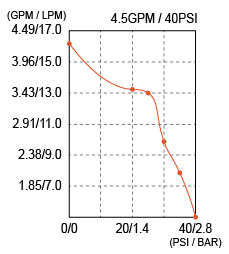
\includegraphics[width=0.35\textwidth]{images/seaflo_lpm_psi.png}
    \label{fig:psi_seaflo}
    \caption{Diagramm der Fördermenge gegenüber des Drucks. \cite{seaflo_pump}}
\end{wrapfigure}
Um die Anfangsgeschwindigkeit zu bestimmen, wurde zunächst angenommen, dass die Pumpe nahe ihrer maximalen Leistung betrieben wird. Diese Annahme basiert auf den Tests mit der zwei Millimeter Öffnung, bei denen auch die Druckabschaltung der Pumpe getestet wurde. Dabei wurde festgestellt, dass die Pumpe nahe der Druckabschaltung von etwa 2,8 Bar betrieben wird.
\\
Basierend auf dem Diagramm in Abbildung \ref{fig:psi_seaflo} lässt sich ableiten, dass die Pumpe bei dieser Einstellung eine Fördermenge von etwa 5 Litern pro Minute haben sollte. Mit diesen Daten kann die Austrittsgeschwindigkeit des Wassers berechnet werden. Dafür wird lediglich der Volumenstrom und der Querschnitt des Laufs benötigt. Allerdings ergibt die Formel $Geschwindigkeit = \frac{Volumenstrom}{Strömungsquerschnitt}$ aus \cite{stroemungen} keine korrekte Berechnung der Austrittsgeschwindigkeit, da ein Wert von über 265 Metern pro Sekunde berechnet wird. Es ist sehr wahrscheinlich, dass die Geschwindikeit durch den Luftwiderstand stark reduziert worden ist.
\\
Daher ist erneut die Formel für den \textit{schrägen Wurf} verwendet worden und nach der Anfangsgeschwindigkeit aufgelöst worden. Dabei stellte sich heraus, das die Anfangsgeschwindigkeit in etwa 10 Meter pro Sekunde beträgt.

Mit diesen Daten ist nun ein präzises anvisieren des Ziels möglich.

\subsection{Ansteuerung}

Zum Testen aller Funktionalitäten ist ein Arduino UNO verwendet worden. Der Arduino kann problemlos verwendet werden, um die Transistoren zu schalten und die Servomotoren zu steuern, da alle erforderlichen Bibliotheken bereits auf dem Board vorhanden sind. Der Testcode kann im Anhang unter \ref{list:Arduino_Test} eingesehen werden.
\\
Der Arduino schaltet alle Aktoren - Ton, Licht, Pumpe und Servomotoren - in bestimmten Zeitabständen ein und aus. Währenddessen werden die Servomotoren in inkrementellen Schritten angesteuert und ein Hochfrequenzton an zwei Pins ausgegeben. Bei diesen Tests stellte sich jedoch heraus, dass der erzeugte Ton zu leise war, um die Tiere effektiv zu stören. Daher wurde eine Verstärkerplatine hinzugefügt, die eine Ausgangsleistung von bis zu zehn Watt ermöglicht. Aus den Informationen von \cite{am_sound_amp} geht hervor, dass die Platine direkt ohne Spannungswandler von der Autobatterie mit Strom versorgt werden kann.
\\
Der Verstärker verfügt über einen Klinkenanschluss. Da der \textit{Jetson Nano} keinen Klinkenanschluss besitzt, wird ein USB-auf-Klinke-Adapter benötigt, um einen Ton abspielen zu können.

Der Jetson Nano besitzt 40 \ac{GPIO} Pins, mit denen die Transistoren geschaltet und die Servomotoren bedient werden können. Der Nano verfügt aber nur über zwei \ac{PWM} Pins. Eine Ansteuerung von mehr als zwei Servomotoren ist daher nicht möglich. \cite{jn_datasheet}

Das Steuern der Aktoren wird durch die von \textit{Nvidia} zur Verfügung gestellte \textit{Jetson.GPIO} Python Bibliothek ermöglicht. \cite{git_jn_gpio}
\\
Damit das Toggeln der Pins die Objekterkennung nicht blockiert, wurde eine threadbasierte Klasse erstellt, die jedem Pin einen eigenen Thread zuweist. Aus dem Hauptprogramm kann das Toggeln jederzeit durch den Befehl \textit{Pin.start\_toggle()} gestartet und durch \textit{Pin.stop()} pausiert werden. Auch kann die Frequenz des Toggelns durch das Multithreading dynamisch in dem Thread selbst verändert werden. Besonders für die Änderung der Schaltfrequenz für das Abschrecklicht eignet sich diese Funktion.
\\
Für die Steuerung der Servomotoren wurde eine ähnliche threadbasierte Klasse erstellt, bei der der Ansteuerungswinkel einfach und ähnlich wie im Arduino-Code aus \ref{list:Arduino_Test} angewendet werden kann.

Beim Testen der Toggle-Funktion wurde jedoch ein irreführendes Verhalten beobachtet. Das Schaltverhalten entsprach nicht immer den Vorgaben. Nach ausführlicher Fehlersuche und einen Blick in das Datenblatt des Jetson Nanos ergab, das die Spannung, die an den meisten \ac{GPIO} Pins anliegt, lediglich 1,8V beträgt und nur teilweise 3,3V. Die ausgewählten Transistortreiber sind jedoch für eine Schaltlogik von 3,3V bis 5V ausgelegt. Zudem wurde im Datenblatt der Transistoren festgestellt, dass bei Verwendung einer 3,3V-Logik der Strom auf unter 10 Ampere begrenzt werden sollte, da sich der Transistor sonst möglicherweise nicht abschalten lässt. Dieses Verhalten konnte beim Betrieb der Wasserpumpe festgestellt werden, da sie sich nur stark verzögert ausschaltete.
\\
Es traten noch weitere Probleme bei der Verwendung der \ac{PWM}-Steuerung der Servomotoren auf. Es schien, als ob die Servomotoren kein gültiges Signal vom Nano erhielten und keinerlei Bewegung zeigten. Bei der Messung der \ac{PWM} stellte sich heraus, dass keine \ac{PWM} erzeugt wurde. Selbst die Troubleshooting-Anleitungen von Nvidia brachten keine Lösung. In einigen Fällen wurde sogar versucht, wie von Nikola Jelic in \cite{forum_wrong_pwm} beschrieben, Registereinträge auf dem Nano vorzunehmen. Leider führten auch diese Versuche nicht zum gewünschten Erfolg. Daher muss für die Steuerung der Servomotoren eine alternative Lösung gefunden werden.
\\
Doch durch den Versuch die \ac{PWM} auf den Nano zu verwenden traten noch weitere Nebeneffekte auf. Das Toggeln der Pins war nicht mehr bis zum neustarten des Nanos möglich. Deshalb wurde die gesamte Hardwareansteuerung auf den Arduino UNO ausgelagert. Dieser hatte sich bereits durch den Funktionstest bewährt.

Für die Ansteuerung der Aktoren durch den Arduino wurde das Testprogramm aus \ref{list:Arduino_Test} angepasst. Der Arduino kann nun über den seriellen Port (USB) Befehle und Werte für die Steuerung des Zielsystems empfangen. Das Toggeln der Aktoren liegt vollständig in der Verantwortung des Arduino. Sobald er Werte für die Ansteuerung der Servomotoren erhält, wird er aktiv und steuert die Aktoren an. Die Steuerung wird solange ausgeführt, bis das Kommando "`g"' vom Nano empfangen wird. Das "`g"' steht dabei für \textit{gone} und signalisiert, dass das Ziel den Zielbereich verlassen hat.
\\
Auf der Seite des Jetson Nanos wurde außerdem eine threadbasierte Steuerung für den Arduino entwickelt. Die serielle Kommunikation mit dem Arduino benötigt deutlich mehr Zeit als die vorherige direkte Ansteuerung über die \ac{GPIO}-Pins, weshalb das Multithreading unbedingt erforderlich ist. Der Effekt auf die zeitliche Interferenz mit der Objekterkennung ist jedoch gering und es konnte keine signifikante Verbesserung durch das Multithreading festgestellt werden.

Den gesamten Schaltplan können Sie in Abbildung \ref{diag:all} einsehen. Die Kamerasensoren werden über den Jetson Nano betrieben und ihre Steuerung erfolgt hauptsächlich über Software. Daher werden sie erst in den nachfolgenden Kapiteln genauer beschrieben.

\begin{figure}[h]
    \centering
    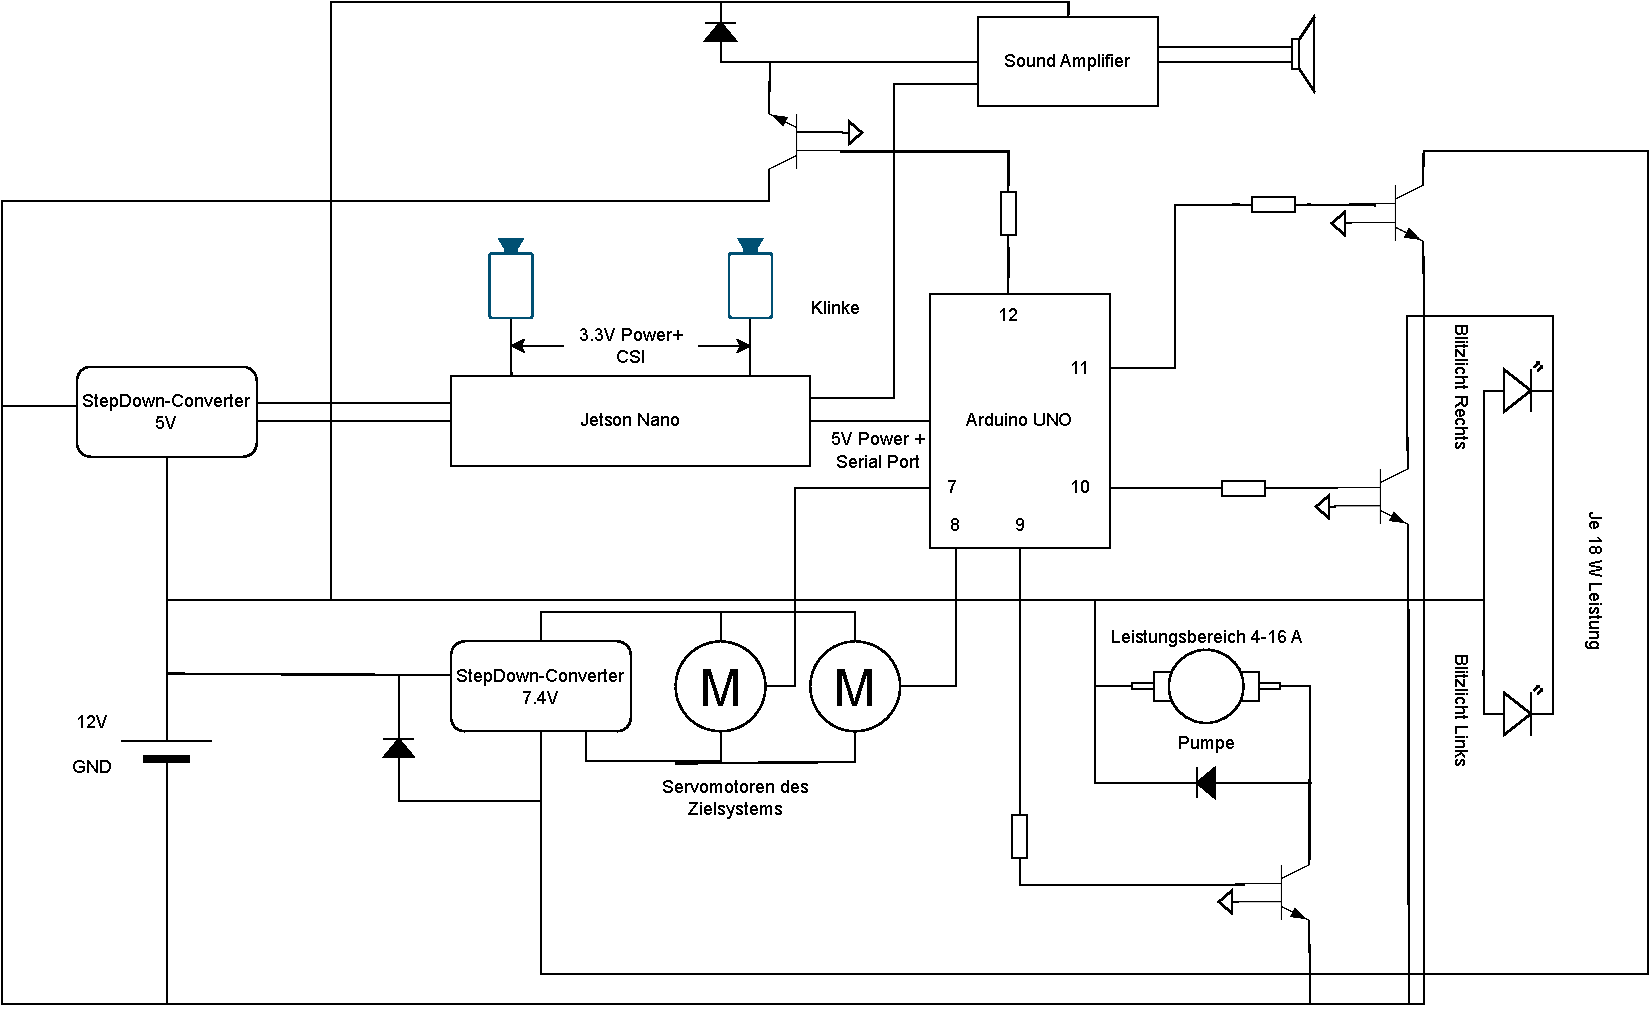
\includegraphics[angle=90,width=0.9\textwidth]{images/Schaltskizzen-Seite-3.drawio.pdf}
    \label{diag:all}
    \caption{Schaltplan der Hardware}
\end{figure}

\section{Objekterkennung und -Verarbeitung}

Der Haupteil der Arbeit bestand in der Entwicklung der Software, insbesondere der Implementierung der Objekterkennung und der Interaktion und Synchronisation der Kameras. Für das Training und Deployment der Objekterkennung wurden hauptsächlich Frameworks verwendet. Dennoch wurden auch einige Hilfsprogramme entwickelt und eingesetzt, welche im Folgenden beschrieben werden.

\subsection{Objekterkennung}

Für die Objekterkennung wurden verschiedene Modelle verwendet. Darunter zwei Modelle aus dem \textit{TensorFlow Model Zoo} und ein Modell von Google für ihren USB-Accelerator \textit{Coral}.
\\
Überwiegend wurde jedoch mit dem \textit{YOLOv8}-Objekterkennungsmodell gearbeitet. Dieses Modell bot klare Vorteile gegenüber den anderen Frameworks. Insbesondere das sehr einfache Setup für das Training sowie die Exportmöglichkeit in verschiedene \ac{ML}-Formate überzeugten. Eine detaillierte Beschreibung dieser Vorteile wird im weiteren Verlauf gegeben.

\subsection{Ordner- und Datenstruktur}

\subsubsection{Sammlung der Trainingsdaten}

Zu Beginn der Arbeit wurde zunächst nach vergleichbaren Modellen und Datensätzen für die \textit{Objekterkennung} gesucht. Dabei fiel auf, dass es für einige unliebsame Kleintiere wie den \textit{Marder} leider keine geeigneten Datensätze gab.

Es gab jedoch bereits ein Modell für die Objekterkennung von Waschbären. Dat Tran hatte im Jahr 2017 ein TensorFlow-Lite-Modell für die Erkennung von Waschbären erstellt. Allerdings hatte er bei der Entwicklung eine andere Absicht. Die Tiere waren seine Lieblingstiere und er wollte wissen, wann ein Waschbär vor seiner Haustür auftaucht.
\cite{wasch_detect}

Mit etwas anderer Absicht lässt sich dies aber auch für die Studienarbeit nutzen, da Dat Tran seine 200 handgelabelten Bilder online zur Verfügung gestellt hat. Diese können für die Objekterkennung des Waschbären verwendet werden und dienen als Grundlage für das Training des Modells in der vorliegenden Arbeit.\\
Die Anzahl der Bilder erscheint für eine erste Betrachtung und Einarbeitung in das Trainieren eines eigenen Objekterkennungsmodells als geeignet. Ein Vergleich der Trainingsmodelle kann in Kapitel \ref{cap:Benchmarks} eingesehen werden.

Der Marder und der Waschbär waren aber nicht die einzigen Tiere, die aus dem Garten ferngehalten werden sollten. Auch Katzen, Füchse und Eichhörnchen sollten aus dem Garten ferngehalten werden. Die Absicht, Katzen und Eichhörnchen fernzuhalten, begründet sich damit, dass wir Vogelliebhaber sind und verhindern möchten, dass diese Tiere die Vögel stören oder ihnen schaden.
\\
Bei den Füchsen sieht es ähnlich aus. Sie sollen von den heimischen Beeten ferngehalten werden, da sie bekanntermaßen Krankheiten übertragen können und somit eine potenzielle Gefahr darstellen.

Um auch Marder und andere Tiere in die Erkennung aufzunehmen, wurden mehrere Datenlabeling-Programme getestet. Das Programm \textit{Label Studio} hat dabei am meisten überzeugt.
\\
\textit{Label Studio} bietet einen interaktiven Workflow und ermöglicht die Zusammenarbeit mehrerer Personen an einem Projekt. Tasks können verschiedenen Personen zugewiesen und übersichtlich dargestellt werden. Die benutzerfreundliche Drag-and-Drop-Oberfläche erleichtert das Labeln von Bildern und das Zeichnen von Bounding Boxes. Ein Beispiel für das Labeln eines Bildes wird in Abbildung \ref{fig:label_studio} exemplarisch dargestellt. Es ist jedoch zu beachten, dass das Bild bereits zu einem späteren Zeitpunkt der Studienarbeit stammt, bei dem das Abschrecksystem bereits funktionsfähig ist. \cite{labelstudio}

Die gelabelten Daten stehen anschließend in dem XML-basierten \textit{Pascal VOC} Datenanotierungsformat zur Verfügung.

\begin{figure}[h]
    \centering
    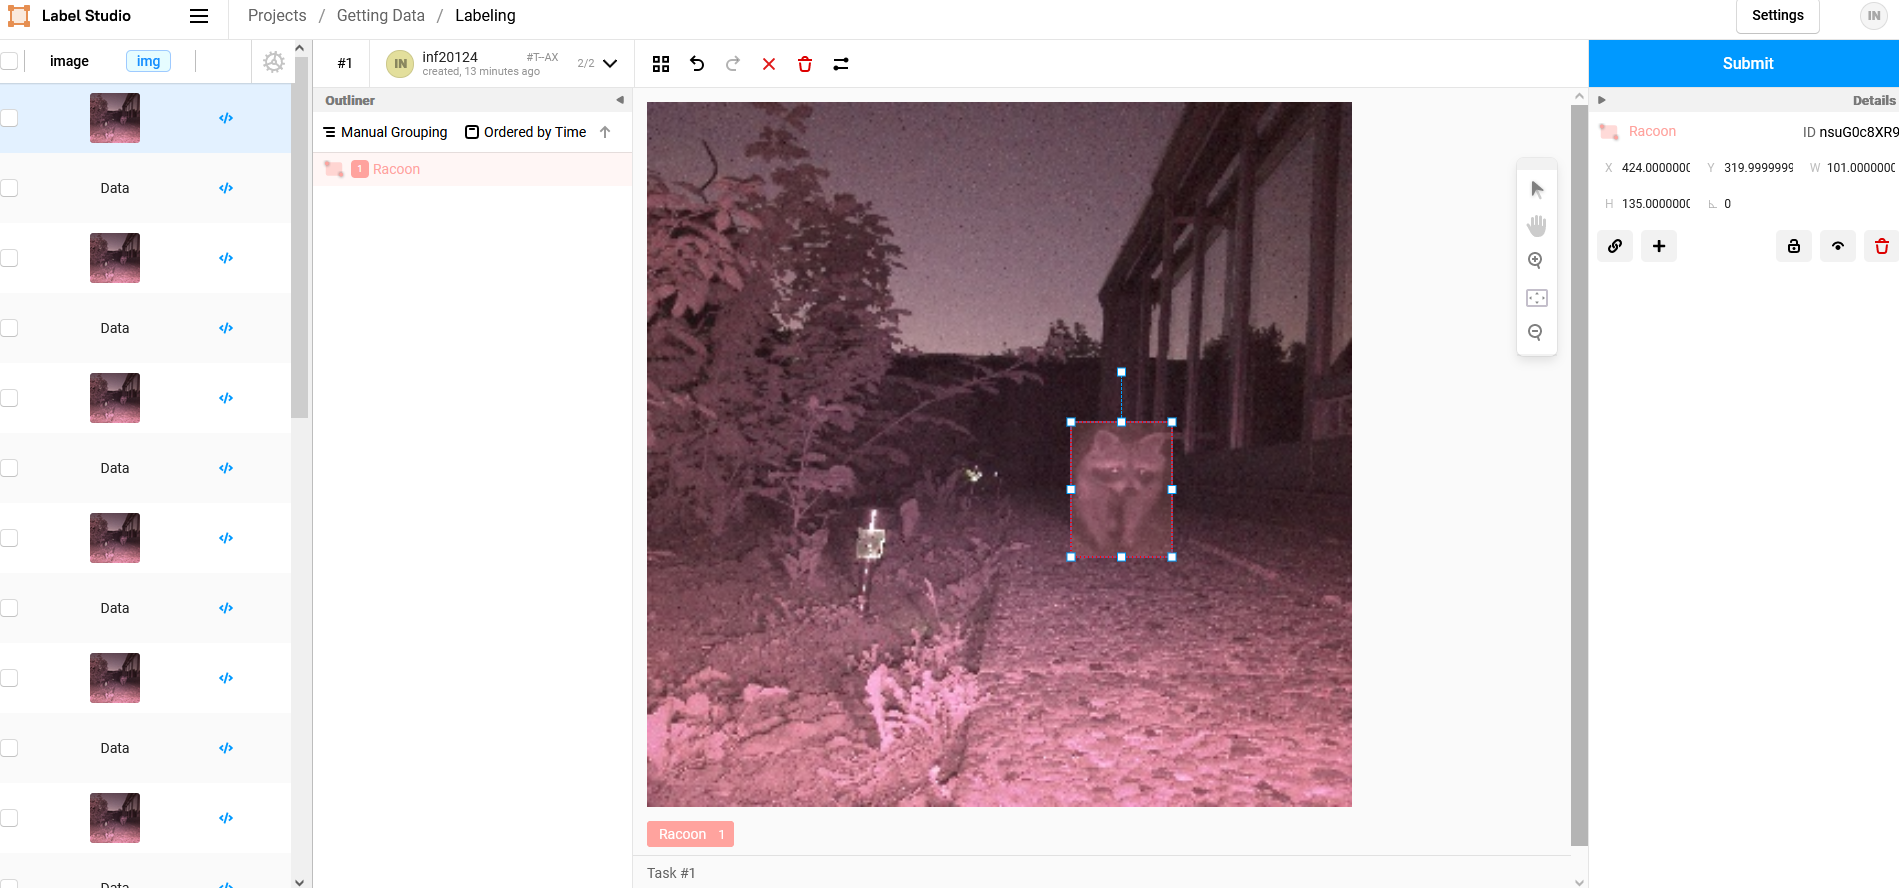
\includegraphics[width=\textwidth]{images/label_studio.png}
    \label{fig:label_studio}
    \caption{Einzeichnen einer Bounding Box mit dem Programm Label Studio}
\end{figure}

Das Problem beim manuellen Erstellen solcher Datensätze ist jedoch, dass dies viel Zeit in Anspruch nimmt. Ein ausreichend großer Datensatz kann daher innerhalb des vorgegebenen Zeitrahmens nicht erstellt werden. Aus diesem Grund wurde die Suche nach zusätzlichen Datensätzen erneut aufgenommen.
\\
Dabei stachen die Daten von \textit{Google Open-Images-V7} heraus. Der Datensatz enthält 16 Millionen Bounding Boxes auf 1,9 Millionen Bildern. Von den 600 verfügbaren Klassen sind auch die für die Arbeit relevanten Tiere enthalten. Allerdings ist ihre Verteilung ungleichmäßig. Ein Großteil der relevanten Bilder handelt von Katzen, während es weniger als tausend Bilder von Waschbären gibt. Daher ist zu erwarten, dass die Waschbären im Endprodukt schlechter erkannt werden als die Katzen. \cite{google_oi7}

Von den 1,9 Millionen Bildern in \textit{Google Open-Images-V7} sind nur etwa 17.000 für das Abschrecksystem relevant, da sie Waschbären, Katzen, Füchse oder Eichhörnchen enthalten. Nur diese Bilder sollten dem Datensatz hinzugefügt werden.
\\
Hier kommt \textit{FiftyOne} ins Spiel. \textit{FiftyOne} ist eine Open-Source-Bibliothek und Plattform zur Datenanalyse von Computer-Vision-Modellen. Eine Funktion von \textit{FiftyOne} ist das Extrahieren und Herunterladen von Computer-Vision-Datensätzen.
\\
Allerdings werden die Bilder und Bounding Boxes nicht getrennt von den nicht benötigten Daten heruntergeladen. Stattdessen werden CSV-Dateien heruntergeladen, die alle Bounding Boxes aufgeteilt in Train-, Test- und Devset enthalten. Diese CSV-Dateien werden anschließend von \textit{FiftyOne} ausgewertet, und die entsprechenden Bilder werden nachträglich heruntergeladen. \cite{fiftyone}

Das Herunterladen der Bilder kann je nach Bandbreite des Netzanbieters eine sehr lange Zeit in Anspruch nehmen. Besonders da die Größe der CSV-Datei, die alle Trainingsdaten beschreibt, bereits mehr als 2,1 GB groß ist. Zusätzlich zur Download-Zeit der CSV-Dateien kommt die Auswertungszeit hinzu, um festzustellen, welche Bilder heruntergeladen werden sollen, sowie die Download-Zeit der eigentlich ausgewählten Bilder.
\\
Nach dem Herunterladen der ausgewählten Bilder und den dazugehörigen Bounding Boxes steht der Datensatz immer noch nicht direkt zur Verwendung bereit. Die Bounding Boxes sind zwar vorhanden, jedoch sind sie weiterhin mit allen anderen Bounding Boxes kombiniert. Dabei beträgt die Größe der CSV-Datei für die Trainingsdaten 2,1 GB, was der Hälfte des Speicherplatzes der heruntergeladenen Bilddaten entspricht.
\\
Weitere Schritte sind daher erforderlich, um den Datensatz für das Training verwenden zu können. Unter dem Skriptordner ist daher ein in \textit{Rust} geschriebenes Konvertierungsprogramm mit der Bezeichnung \textit{csv\_conv} abgelegt. Dieses Skript konvertiert die heruntergeladenen CSV-Dateien in ein CSV-Format, das mit \textit{TensorFlow} kompatibel ist. Dabei werden auch alle nicht relevanten Bilddaten und Bounding Boxes herausgefiltert. Die Größe der resultierende CSV-Datei, die alle Trainings-, Test- und Devset-Bounding Boxes enthält, beträgt danach weniger als 1 MB.\\
Zusätzlich wurden irrelevante Daten entfernt, wie die Datenquelle sowie die Informationen \textit{IsOccluded, IsTruncated, IsGroupOf, IsDepiction, IsInside} und die \textit{Confidence}. Die \textit{Confidence} gibt an, mit welcher Wahrscheinlichkeit ein Objekt erkannt wurde. Jedoch spielt dieses Feld nur eine Rolle, wenn ein Objekterkennungsmodell die Bounding Box vorhersagen würde. Da dies bei den vorliegenden Daten nicht der Fall ist, kann das Feld ebenfalls gelöscht werden.
\\
Durch die Deserializierung können diese Felder automatisch ohne Mehraufwand in der Programmierung entfernt werden.
Als ein letzter Schritt werden danach die Bounding Box Daten, welche in Prozent angegeben sind, in eine Ganzzahl konvertiert und die Klasse des Objektes von einer ID zu einem Namen (zum Beispiel \textit{Racoon}) aufgelöst.

Nun gibt es jedoch ein weiteres Problem: Die Daten von Dat Tran und die von \textit{Google-Open-Images} liegen in unterschiedlichen Dateiannotierungsformaten vor. Allerdings hat Dat Tran in \cite{wasch_detect} bereits ein Python-Skript mit dem Namen \textit{xml\_to\_csv} erstellt, das die XML-Dateien in eine CSV-Datei konvertiert. Dieses Skript wurde an dieser Stelle verwendet und befindet sich ebenfalls im Skriptordner.

Mit den nun vorliegenden Daten kann die Objekterkennung angegangen werden.

\subsubsection{Training}

\subsubsection{Deployment}

 Auch mit random 0 Byte Bilddaten/ fehlende XML-Dateien /leere XML-Dateien und das diese für weiteres Training verwendet werden können. Warum XML? Konvertierungsskript vorhanden, sowie falls 0 Byte Fehler wärs bissle schaud für der rest, weil die dann au weg wäred
\subsection{Benchmarks} \label{cap:Benchmarks}

\subsubsection{Interferenzzeit}

\subsubsection{Erkennungsqualität}

\subsection{Erkennung durch Kontur-tracking}

\subsection{Verbesserung der Bildqualität}

\subsection{Tiefenberechnung} \label{cap:calc_depth}

\section{Kostenaufstellung}

\begin{longtable}{ p{0.15\textwidth}|p{0.2\textwidth}|p{0.5\textwidth} }
    \endfirsthead
    \multicolumn{2}{l}%
    {\textit{Fortsetzung von vorheriger Seite}} \\
    \hline
    \endhead
    \hline \multicolumn{2}{r}{\textit{Fortsetzung auf nachfolgender Seite}} \\
    \endfoot
    \endlastfoot
    \textbf{Bauteil} & \textbf{Gesamtpreis in € (inkl. Mwst.)} & \textbf{Beschreibung}\\
    \hline
    LED-Scheinwerfer
    & \centering11.99
    & Die effizienten LED-Scheinwerfer sind für die Anwendung als Erweiterungsleuchten für das Fahrzeug gedacht. \cite{am_licht} Da die LEDs den hohen Belastungen beim Einsatz am Fahrzeug standhält, werden sie den Anforderungen an einem portablem Abschrecksystem gerecht. Sie werden als Blitzlicht für das Abschrecksystem verwendet.
    \\
    Membran-pumpe
    & \centering73.35
    & Membranpumpen sind bei einfachen und kostengünstigen Anwendungen vertreten. Durch den geringen Verschleiß und einfache Wartbarkeit werden sie häufig in Frisch- und Abwasseranwendungen eingesetzt. \cite{mebranpumpe} In der Arbeit wird die Pumpe wegen ihrem geringen Verschleißes und Anschaffungskosten verwendet.
    \\
    Solarpanel
    & \centering69.99
    & Das Solarmodul wird verwendet um die Portabilität und Autarken Eigenschaften der Abschrecksystems zu gewährleisten. Solange Sonnenlicht am Einsatzort verfügbar ist, kann das Abschrecksystem mit ausreichend Energie versorgt werden um die unliebsamen Kleintiere zu erkennen.
    \\
    Autobatterie
    & \centering59.90
    & Kombiniert mit dem Solarmodul versorgt die Batterie das Abschrecksystem mit der nötigen Energie. Tagsüber wird sie mithilfe des Solarmoduls aufgeladen, während sie Nachts das System mit Energie versorgt. \cite{Autobatterie}
    \\
    Diverse Kleinteile
    & \centering{25 + X}
    & Diverse Kleinsteile werden in der Arbeit verwendet. Auch die Transistoren, die verwendet werden um die verschiedenen Aktoren an- und auszuschalten fallen unter dieser Kategorie. Aber auch die Räder, Schläuche, Kabel, Steckverbindungen und Schrauben werden hier miteinberechnet. Zusätzlich kommen die, für das Abschrecksystem angefertigten 3D-gedruckten Elemente hinzu.
    \\
    Aluminium-kiste
    & \centering{109 DM}
    & Die Aluminiumkiste ist Witterungsfest und besitzt eine gute Wärmeableitung. Alle Aktoren und Gerätschaften können in ihr vor Witterungsbedingungen geschützt untergebracht werden.
\end{longtable}

\begin{figure}
    \centering
    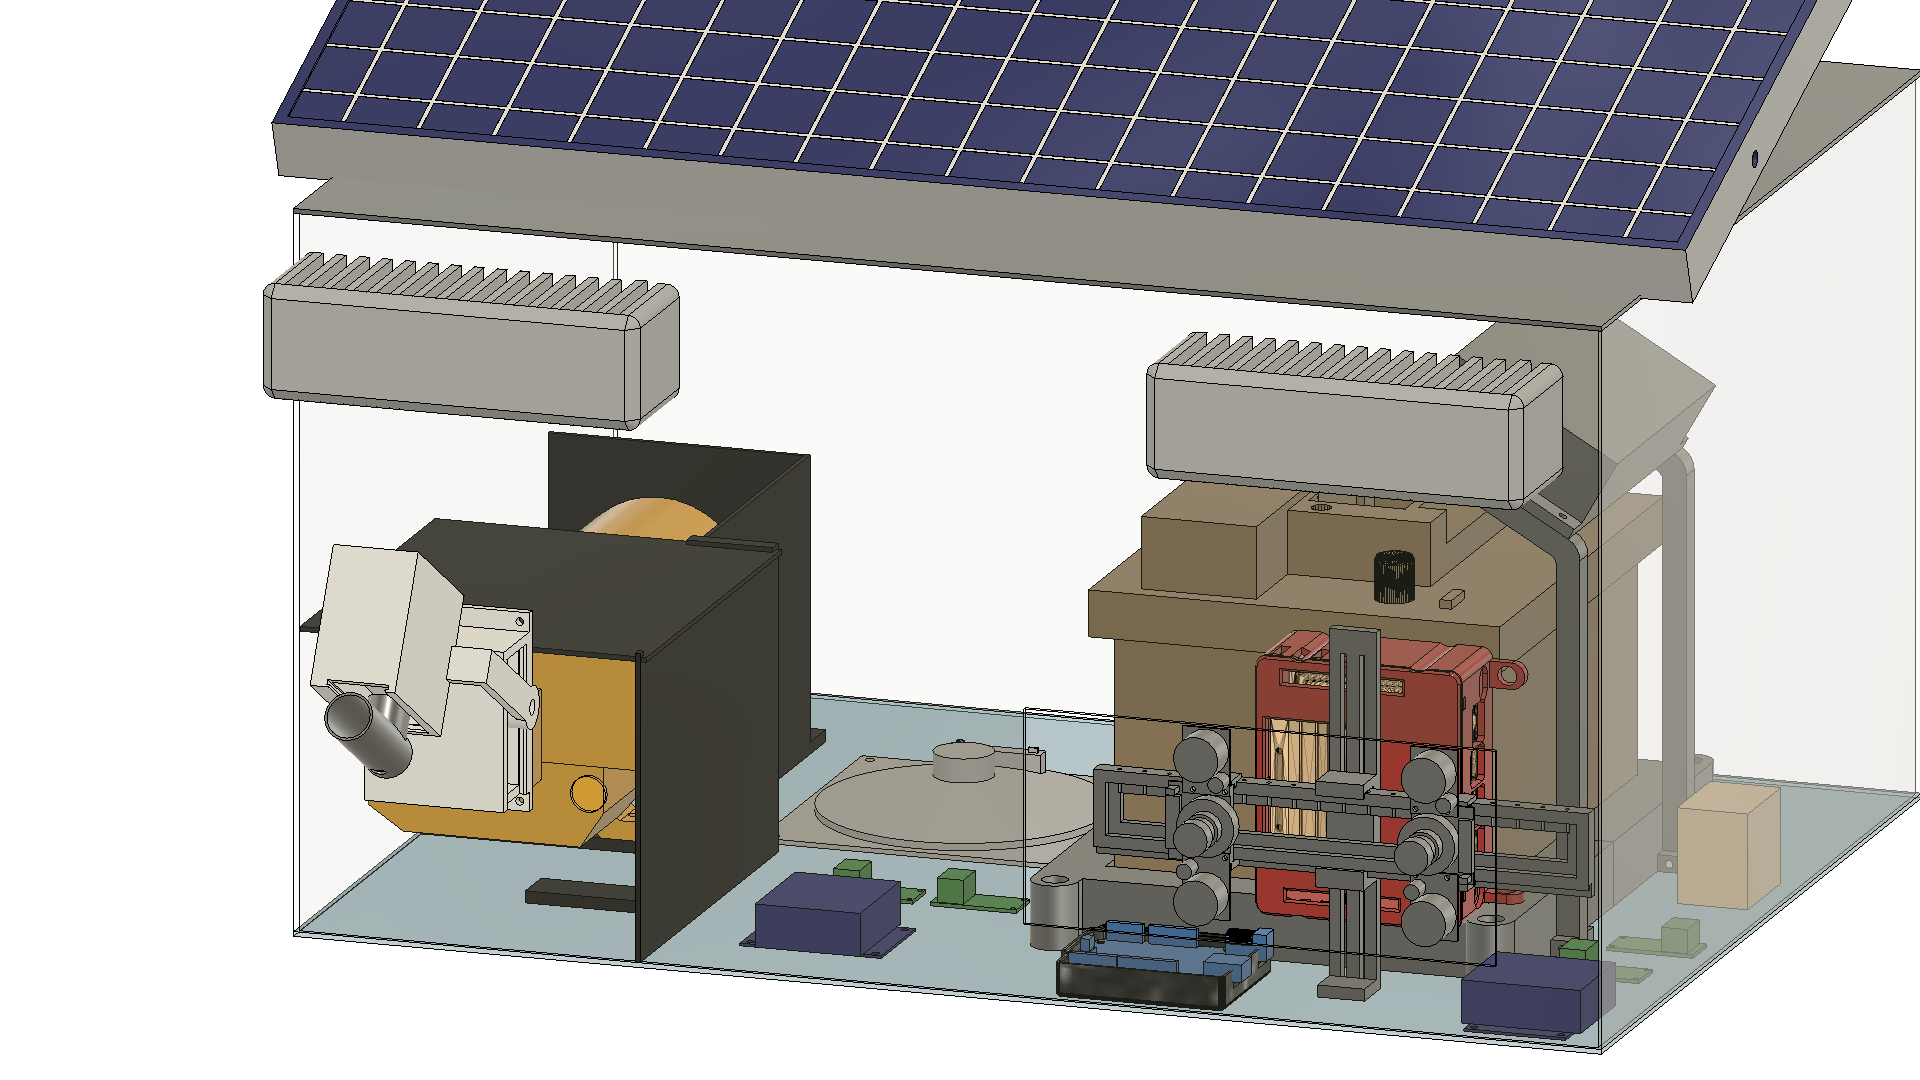
\includegraphics[width=\textwidth]{images/whole_box.png}
    \label{fig:whole_thing}
\end{figure}
